\section{Summary of the method and main results}
\label{sec:summary}
\begin{figure}[h!]
    \centering
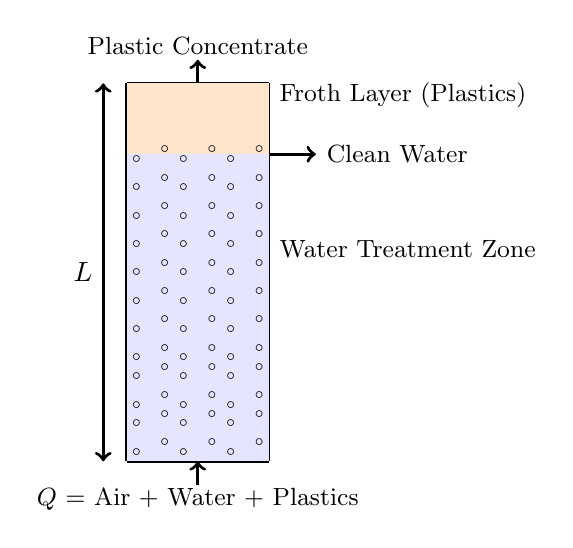
\begin{tikzpicture}[scale=0.6,very thick]

    % Column body
    \draw (0,0) -- (0,8);
    \draw (3,0) -- (3,8);
    \draw (0,8) -- (3,8);
    \draw (0,0) -- (3,0);
    
    % Height label L
    \draw[<->] (-0.5,0) -- (-0.5,8)node[midway, left]{$L$};
    
    % Froth zone (microplastics)
    \fill[orange!20] (0,6.5) rectangle (3,8);
    \node[right] at (3,7.75) {\small Froth Layer (Plastics)};
    
    % Water treatment zone
    \fill[blue!10] (0,0) rectangle (3,6.5);
    \node[right] at (3,4.5) {\small Water Treatment Zone};
    
    % Air+Water+Plastic inlet
    \draw[ ->] (1.5,-0.5) -- (1.5,0);
    \node at (1.5,-0.8) {\small $Q$ = Air + Water + Plastics};
    
    % Clean water outlet (side)
    \draw[ ->] (3,6.5) -- (4,6.5);
    \node[right] at (4,6.5) {\small Clean Water};
    
    % Plastic concentrate outlet (top)
    \draw[ ->] (1.5,8) -- (1.5,8.5);
    \node at (1.5,8.8) {\small Plastic Concentrate};
    
    % Bubbles
    \foreach \y in {1.2, 1.8,0.2, 0.8,2.2, 2.8, 3.4, 4.0, 4.6, 5.2, 5.8, 6.4} {
      \node at (1.2,\y) {\tiny $\circ$};
      \node at (1.8,\y+0.2) {\tiny $\circ$};
      \node at (0.2,\y) {\tiny $\circ$};
      \node at (0.8,\y+0.2) {\tiny $\circ$};
      \node at (2.2,\y) {\tiny $\circ$};
      \node at (2.8,\y+0.2) {\tiny $\circ$};
    }
\end{tikzpicture}
\caption{Sketch of a typical flotation column with high $L$. The input flow rate $Q$ is usually imposed by the upstream processes.  The goal of this study is then to predict the output of ``Plastic concentrate''  and the high $L$ in terms of the input flow rate $Q$. }
\end{figure}


\subsection{Definitions}
Let us first introduce a series of dimensionless numbers: 
\begin{align*}
    \xi = d_b / d,
    && L^* = L / d,
    && \zeta = \rho_b / \rho_f,
    && \lambda = \mu_b / \mu_f,\\
    \phi_b = V_b/V_{tot},
    && \phi_p = V_p/V_{tot}.
    && \phi_p^a = V_p^a/V_{tot}.
    && X\% = \phi_p^a /\phi_p\\
    &&
    Re = |\textbf{u} - \textbf{u}_b|\rho_f d /\mu_f ,
    && Ga = d^3 g\rho_f^2 (1-\zeta)/\mu_f^2. 
\end{align*}
$d$ and $d_p$ are the diameter of the spherical bubbles and particles, respectively.
$L$ is the height of the flotation column. 
$\mu_k$  and $\rho_k$ are the viscosity and density of the phase $k$. 
Hence, $\lambda = 0$ corresponds to the case of clean bubbles, while $\lambda \to\infty$ represents fully contaminated bubbles, characterized by a no-slip condition at their interfaces.
$V_k$ is the total volume of phase $k$. 
$V^a_k$ corresponds to the volume of attached particles (number of attached particles times the volume of a single particle). 
``$k$'' represents either the bubbles phase ($k=b$), the water phase ($k=f$), or the particles phase ($k=p$).
$g = 9.81$ m.s$^{-2}$ represents the gravity acceleration. 
$\textbf{u} = \phi_p \textbf{u}_p + \phi_b \textbf{u}_b + \textbf{u}_f(1-\phi_b+\phi_p)$ represents the velocity of the mixture, $\textbf{u}_k$ being the mean velocity of phase $k$.

With these definitions $Ga$ is the \textit{Galileo} number, comparing viscous to buoyancy forces, and $Re$ is the bubbles Reynolds number, comparing viscous drag force and inertial forces acting on the bubbles.
$\phi_k$ the volume fractions of each phase. 
And $X\% $ the percentage of attached particles in the column. 

The objective of this study is to determine $L^*$ for a given $X\%$.
In the ideal scenario we would like to clean $100\%$ of waste in the water, this corresponds to $X\%=1$, however we will see that due to the asymptotic behavior of the function $L^* (X\%)$ one may only be able to reach $X\% \approx 0.9$ in order to keep a height $L$ of the order of a meter. 

\subsection{Governing equations}

In a first modeling attempt, we need to state a considerable number of assumptions. 
These will be relaxed in future studies however for instance we consider that:
\begin{enumerate}
    \item The flow (meaning the bulk and bubbles and particles velocity) is established along the columns and at steady-state.
    \item Plug flow: $\textbf{u}$, $\textbf{u}_b$ and $\textbf{u}_p$ are constant across the section. That means that we neglect the effects of the sides of the column on the flow.
    \item The two previous hypotheses also apply to the concentration fields $\phi_k$. 
    However, $\phi^a_p$ varies along the column height as bubbles catch free particles in the flow while rising. 
    \item $\phi_p\ll \phi_b<0.25$ and $Ga<100$ : This is not too restrictive as in the real processes these criteria are often respected. 
    \item $\xi \ll 1$: The collision efficiency is computed such that we neglect the $O(\xi^3)$ (see~\ref{sec:efficiency}) term hence $\xi$ must be reasonably low. 
    \item $Re_p\ll 1$: Due to their small size, the particles are considered inertialess, such that they can be assimilated to tracers in the ambient fluid. 
    \item In this study, we focus exclusively on the collision mechanism and disregard both the detachment phenomenon and the probability of attachment. 
    We assume that the probability of attachment is equal to 1, meaning that every collision between bubbles and particles results in attachment.
\end{enumerate}

With these assumptions in hand the modeling process goes into two steps: compute the hydrodynamic of the bubbles and water, then consider the particles as an independent phase evolving according to the velocity field \textbf{u} but without backward interaction (one way coupling). 
This is allowed thanks to the very small volume fraction of particles $\phi_p^a$, usually below 1~\textperthousand{}

Assuming $x$ is the coordinates along the column axis, the mass and momentum averaged equations applied to a two phases system (made of bubbles and water) read as, 
\begin{align}
    \label{eq:divu_zero}
    \pddx \textbf{u} &= 0 \\
    \pddx \phi_b &= 0 \\
    \label{eq:ur}
    C_d(Re,\lambda,\phi_b) &= \frac{4(1-\phi_b)^3}{3}\frac{Ga}{Re^2} \Longleftrightarrow  \textbf{u}_b = \textbf{u}  + F(\lambda , Ga, \phi_b)
    % \textbf{u}_p &= \textbf{u} \\
    % L &= 
    % - \frac{2}{\phi_b 3(1+\xi)^2}
    % \frac{u_b^S}{\left|\textbf{u}_p  - g(\lambda,\xi)\textbf{u}_b\right|^S}
    % \ln(1 - X\%)
\end{align}
The first equation simply states that the mixture velocity as well as the bubbles' volume fraction are conserved, see~\ref{sec:averaged_equations}. 
\ref{eq:ur} is the ``relative averaged momentum'' equation, it is to be solved for $\textbf{u}_b$ which is hidden inside the $Re$ variable. 
This equation expresses the balance between buoyancy forces (represented in dimensionless form by $Ga$) and hydrodynamic drag force (represented by the drag coefficient $C_d$). 
Note that $C_d$ is the drag coefficient for emulsion which is given in \citet[Chapter 8]{fintzi2025} and in~\ref{sec:averaged_equations}.
Here, $F(\lambda,Ga,\phi_b)$ represents a symbolic function that is actually computed numerically with the attached \texttt{python} script (see~\ref{ap:python}). 

The particles' velocity as well as the volume fraction of attached particles, is given by:
\begin{align}
    \textbf{u}_p &= \textbf{u}\\
    \pddt \phi_p^a  + \pddx (\textbf{u}_b \phi_p^a)
    &= 
    (\phi_p - \phi_p^a) \Gamma
    \label{eq:kinetic_summary}
    \\
    \Gamma &= \phi_b \frac{3(1+\xi)^2 }{2d}
    \left|\textbf{u}_p  - \textbf{u}_b + g(\lambda,\xi) (\textbf{u} - \textbf{u}_b)\right|\\
    g(\lambda,\xi)
    &=
    -1+\frac{\xi}{\lambda + 1} + \xi^2  \frac{6\lambda - 2}{3(\lambda+1)}
    + O(\xi^3).
    % \label{eq:final_Ec}
\end{align}
Recall that $\phi_p^a$ is the volume fraction of attached particles, hence $\Gamma$ represents the rate at which particles get attached to bubbles in [s$^{-1}$], and $g(\lambda,\xi)$ the so-called ``collision efficiency'' \citep{loewenberg1994flotation}.
Although the derivation of $g(\lambda,\xi)$ remains classic, the results obtained in this study is different from what has been proposed in the literature~\citep{loewenberg1994flotation}, all the details of the derivation are given in~\ref{sec:efficiency}. 

In this model only $\phi_p^a$ is function of the column height, hence one may solve this equation for $\phi_p^a$ and determine for which $x = L^*$ the number of particle attached to bubbles corresponds to $X\%$, or symbolically $\phi_p^a(L^*)/\phi_p = X\%$.
As given in ~\ref{sec:efficiency} the exact expression for $L^*$ is, 
\begin{equation}
    \boxed{
        L^* = 
        - \frac{\textbf{u}_b}{d \Gamma}\ln(1 - X\%).
        }
    \label{eq:L_solution}
\end{equation}
When $X\% \to 1$ we have $L^* \to \infty$ hence our objective is limited to values below $1$. 

\subsection{A few examples}

In the following we use the physical parameters, 
$
    \mu_f = 10^{-3} \;\text{ [kg.m$^{-1}$.s$^{-1}$]}  $  
    $ 
    \rho_f = 10^{3} \;\text{ [kg.m$^{-3}$]},
$
for the water.  
The bubbles generated by dissolved air flotation have $d\approx 70\mu m$. 
Finally, we arbitrarily fix an objective of $X\% = 0.9$ for the processes. 

\subsubsection*{CleanWash:} 
For this flotation column the input mixture flow rate (bubbles + water+ fibers) is, $Q = [2\text{-}4]$[L/min], and the diameter of the column $R = 0.1 m$.
We determine $\textbf{u}$ from $Q$ and $R$ and the condition given by~\ref{eq:divu_zero}. 
The particles are fibers hence our model cannot be applied directly, for instance we consider an equivalent diameter of $d_p = [10\text{-}20]\mu m$. 

Based on the values of $\textbf{u}$, $d$ and $d_p$ we display the corresponding values of $L$ using~\ref{eq:ur} to~\ref{eq:L_solution} for various viscosity ratio $\lambda$ and $\phi_b$, see~\ref{fig:height} (left). 
\begin{figure}[h!]
    \centering
    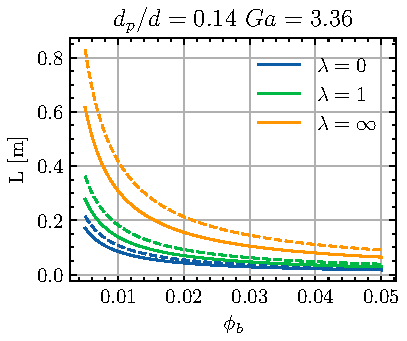
\includegraphics[height=0.40\textwidth]{image/flotation/examples/case_one.pdf}
    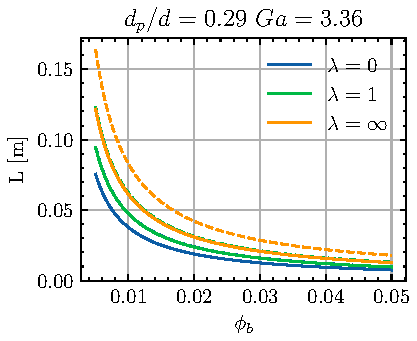
\includegraphics[height=0.40\textwidth]{image/flotation/examples/case_one_xi2.pdf}
    \caption{
    $L$ in meter for various $\lambda$ and $\phi_b$ for the column of CleanWash. 
    (dashed lines) correspond to $Q=4$ [l/min], and (solid line) to $Q = 2$ [l/min].
    (left)$d_p = 10\mu m$
    (right) $d_p = 20\mu m$ to highlight the important role of $xi$ or more generally of $\Gamma$ on $L$. }
    %  COLUMN SOLAIZE:  $L$ in meter for various $\lambda$ and $\phi_b$. (dashed lines) correspond to $Q=0.5$ [l/min] (solid line) $Q = 0.25$ [l/min]  }
    \label{fig:height}
\end{figure}
It is clear from~\ref{fig:height} and from~\ref{eq:L_solution} that $L \sim d/d_p = \phi_b^{-1}$ and that $L \sim  \xi^{-1}$ at the dominant order, hence for small $\phi_b$ and $\xi$, $L$ is very sensitive to those parameters.
Hence, for accurate modeling, one must know the exact values of these parameters in the actual process.  
This is left for a future investigation. 


\subsubsection*{Lab. flotation column at Solaize (2L)}

This flotation column has nearly the same parameters, however the flow rate is $Q= [0.25\text{-} 0.5]$ [l/min]. 
In~\ref{fig:height_two} we display the corresponding $L$. 

\begin{figure}[h!]
    \centering
    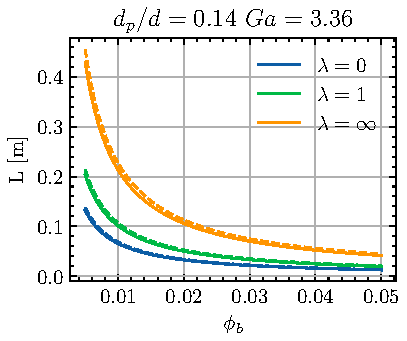
\includegraphics[height=0.40\textwidth]{image/flotation/examples/case_two.pdf}
    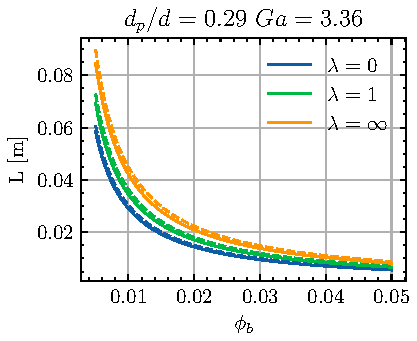
\includegraphics[height=0.40\textwidth]{image/flotation/examples/case_two_xi2.pdf}
    \caption{
    $L$ in meter, for various $\lambda$ and $\phi_b$ for the lab. Flotation column (Solaize). 
    (dashed lines) correspond to $Q=0.5$ [l/min], and (solid line) to $Q = 0.25$ [l/min].
    (left) $d_p = 10\mu m$
    (right) $d_p = 20\mu m$ to highlight the important role of $xi$ or more generally of $\Gamma$ on $L$. }
    %  COLUMN SOLAIZE:  $L$ in meter for various $\lambda$ and $\phi_b$. (dashed lines) correspond to $Q=0.5$ [l/min] (solid line) $Q = 0.25$ [l/min]  }
    \label{fig:height_two}
\end{figure}
Again the results are very sensitive to the value of $\xi$ and $\phi_b$ for the same reason as the previous examples. 
The global height is lower because the mixture flow rate is lower. 
The influence of the viscosity ratio $\lambda$ on $L$ also seems important, hence it is primordial to know whether or not the bubbles are contaminated ($\lambda \gg 1$) or clean ($\lambda \ll 1$).

\vspace{0.5cm}
\noindent
\fbox{
    \begin{minipage}{\textwidth}
        Overall if we assume that dissolved air flotation produces a flow rate of bubbles equivalent to $\phi_b = 0.01$ then the required length for the column is $L \approx 0.2$ m, if we take $d_p = 10\mu m$ and $\lambda =\infty$ which is the most probable scenario. 
    \end{minipage}
        }
    

\subsection{Perspectives}

Regarding the improvement of the theory first:
We think that it would be nice in a future study to relax the hypothesis 2., 3., and 6. of the list mentioned above since it is rather strong and not verified assumptions. 
Regarding the development of the collision kernel the Perspectives of improvement are summarized at the end of~\ref{sec:efficiency}. 

In the actual flotation process it seems that the flow rate $Q$ is a related to $\phi_b$ hence these two parameters are linked, this must appear in the next study. 
It would be also interesting to investigate more complicated column geometries and how this is related to the global efficiency of the process. 


% In the first place we apply this model on \textbf{Clean Wash}, however it would be nice to investigate the ``\textbf{P-FAS} column'' and the one use for \textbf{battery recycling} with the same modeling approach. 


Here, we first apply this model to the CleanWash geometry in the presence of solid particles. 
However, the model could be adapted to other cases, in particular to flotation geometries used for battery metal recycling (graphite recovery), or even for the recovery of PFAS molecules in foam fractionation processes. 

The python script used to plot those graphs is available in~\ref{ap:python}. 

